\chapter{周期边界情形的可观测性}
    
     本章考虑周期情形的线性KdV方程
    \begin{align}\label{kdv-l}
        \left\lbrace \begin{array}{ll}\partial_t u +\partial_x^3u=0, & (t,x)\in \R\times (0,2\pi), \\
        \partial_x^ku(t,0)=\partial_x^k u(t,2\pi), & 0\le k\le 2,\\
        u(0,x)=u_0(x), & x\in (0,2\pi),
        \end{array}\right.
    \end{align}
       并给出方程 \eqref{kdv-l} (1) 关于一个移动观测点的能观测不等式 (2) 关于两个移动观测点的能观测不等式及判定方法.
    定义该情形下 Sobolev 空间
    \begin{equation*}
        H^3_p:=\lbrace v\in H^3 (0,2\pi):\partial_x^i v(0)=\partial_x^i v(2\pi), i=0,1,2 \rbrace.
    \end{equation*}
    对任意的初始函数 $u_0\in H_p^3$, 存在唯一的弱解
    \begin{equation*}
        u\in C(\R, H^3_p)\cap C^1(\R,L^2(0,2\pi)).
    \end{equation*}
    进而, $u$ 可以表示为
    \begin{equation}
        u(t,x)=\sum_{k\in\Z}c_k e^{i(k^3t+kx)},
    \end{equation}
    其中 $c_k$ 是 $u_0$ 的傅里叶系数:
    \begin{equation*}
        u_0(x)=\sum_{k\in \Z} c_ke^{ikx}.
    \end{equation*}
    一般情形下, KdV 方程都是实值函数, 所以还额外满足 $\overline{c_{-k}}=c_k, \forall k\in \Z$. 接下来的讨论对实值函数与复值函数都适用, 并在一些地方额外加以说明.
    \section{Ingham不等式与Eisenstein整数}
    设 $I$ 为一区间, 且 $|I|=2\pi$, 则我们可以将著名的Parseval公式写作
    \begin{equation*}
        \frac{1}{|I|} \int_I \left| \sum_{k\in \Z} c_k e^{ikx}\right|^2 \d x = \sum_{k\in \Z} |c_k|^2.
    \end{equation*}
    该公式对于 $|I|=2k\pi, k\in \N$ 也正确, 由此易知, 对于任意满足 $2k\pi <|I|<(2k+2)\pi,k\in\N$ 的区间 $I$, 都有
    \begin{equation*}
        2k\pi \sum_{k\in \Z}|c_k|^2 \le \int _I \left| \sum_{k\in \Z}c_ke^{ikx} \right|^2\d x \le (2k+2)\pi  \sum_{k\in\Z }|c_k|^2. 
    \end{equation*}
    自然地, 给定一个区间 $I$, 以及一个实数集 $\Lambda$, 是否存在常数 $c,C>0$, 使得对任意的平方可和序列 $\left\{c_k\right\}_{k\in \Z}$都有关系式
    \begin{equation}
        c \sum_{k\in \Lambda} |c_k|^2 \le \int _I \left| \sum_{k\in \Lambda} c_k e^{ikx} \right|^2 \d x \le C \sum_{k\in \Lambda}|c_k|^2
    \end{equation}
    或其等价形式
    \begin{equation}\label{3-1-2}
        \int _I \left| \sum_{k\in \Lambda} c_k e^{ikx} \right|^2 \d x\asymp \sum_{k\in \Lambda}|c_k|^2,
    \end{equation}
    成立呢? 若成立, 则上式可看作Parseval公式在区间 $I$以及指数集合$\Lambda$ 上的推广. 
    
    为了建立上述Parseval公式的推广, Ingham \cite{Ingham1936} 证明了下述定理
    \begin{theorem}\label{thm-ingham}
    设 $\Lambda$ 为一族实数集, 且该实数族满足条件
    \begin{equation}\label{3-1-1}
        \gamma(\Lambda)=\inf\lbrace |\lambda_1-\lambda_2|: \lambda_1\neq \lambda_2, \lambda_1,\lambda_2\in \Lambda\rbrace>0,
    \end{equation}
     则对任意满足 $|I|>2\pi /\gamma$ 的区间 $I$都有关系式 \eqref{3-1-2} 成立. 实际上, 关系式的常数可以具体给出并写作
     \begin{equation}
         \frac{2\alpha(4\pi+\alpha)}{\pi(2\pi+\alpha)^2}|I|\sum_{k\in\Lambda}|c_k|^2\le \int_{I}\left|\sum_{k\in \Lambda}c_ke^{i\lambda_kx}\right|^2\d x\le \frac{20 |I|}{\min\left\{\pi,|I|\gamma(\Lambda)\right\}}\sum_{k\in\Lambda}|c_k|^2,
     \end{equation}
     其中 $\alpha=|I|\gamma_0-2\pi$.
     
      我们称满足条件 \eqref{3-1-1} 的实数集为一致分离集. 
    \end{theorem}
    
    条件 $|I|> 2\pi /\gamma$ 是对所有满足 \eqref{3-1-1} 实数族的一致最佳条件, 但在某些特殊情形下, 这一条件可以被改进. Haraux \cite{Haraux1989} 给出了下述定理.
    
    \begin{theorem}\label{thm-haraux}
    设 $\Lambda$ 为一致分离集, 且 $F\subset \Lambda$ 为有限子集, 则关系式 \eqref{3-1-2} 在 $|I|> \frac{2\pi}{\gamma(\Lambda \backslash F)}$ 的条件下也成立.
    \end{theorem}
    

    
   
    本章第三节对多条线段的可观测性研究中, 涉及到集合
    \begin{equation}\label{Gamma-set}
        \Gamma:=\lbrace n:\exists m,k\in \Z,m\neq k \text{ s.t. } n=m^2+mk+k^2 \rbrace
    \end{equation}
    中元素的性质. 而该集合在数论中与 Eisenstein 整数相关, 本节旨在介绍 Eisenstein 整数及其与文章内容相关的性质. 对下述提到的环, 数域, 整环, 唯一分解整环, 欧几里得整环等基本概念, 参见. 
    
\begin{definition}
    一个数 $\alpha \in \C$  称为代数数, 若其是一个多项式
    \begin{equation*}
        f(x)=a_nx^n+a_{n-1}x^{n-1}+\cdots+a_1x+a_0
    \end{equation*}
    的跟, 其中 $a_0,a_1,\cdots,a_{n-1},a_n\in \Q, a_n\neq 0$. 
    若, $\alpha$ 不是代数数, 则称其为超越数.
    
    特别地, 若存在多项式系数均为整数且 $a_n=1$, 使得 $\alpha$ 为它的根, 则称 $\alpha$ 为代数整数. 
\end{definition}

\begin{definition}
    若数域 $F$ 包含一个子数域 $k$, 则称 $F$ 是数域 $k$ 的域扩张, 记作 $F /k$. 若 $F$ 是 $k$ 的扩张, 则可以将$F$ 看作域 $k$ 上的线性空间, 该线性空间的维数被称为域扩张的度数并记作
    \begin{equation*}
        [F:k]=\text{线性空间 } F \text{ 在 } k \text{ 上的维数}.
    \end{equation*}
\end{definition}

\begin{definition}
    数域 $\C$ 中的子数域, 称为代数数域, 若其是包含代数数 $\alpha_1,\alpha_2,\cdots,\alpha_n$ 和 $\Q$ 的最小数域, 并记作 $\Q(\alpha_1,\alpha_2,\cdots,\alpha_n)$.
\end{definition}

代数整数推广了整数的概念, 例如有理数域 $\Q$ 中所有的代数整数是 $\Z$, 高斯数域 $\Q(i)$ 中所有代数整数是 $\Z[i]$.

\begin{theorem}
若 $K$ 是一个代数数域, 则存在一个代数数 $\theta$ 使得 $K=\Q(\theta) $.
\end{theorem}

\begin{definition}
    令 $\omega =e^{\frac{2\pi i}{3}}$, 则易知 $\Q (\omega)$ 中的所有代数整数构成的整环为 $Z[\omega]$. 整环 $Z[\omega]$ 称为 Eisenstein 整环, 其中的元素称为 Eisenstein 整数. 记 $\Z [\omega]$ 中的所有可逆元为 $U(\Z[\omega])$, 则
    \begin{equation*}
        U(\Z[\omega])=\lbrace\pm 1,\pm \omega, \pm \omega ^2\rbrace.
    \end{equation*}
\end{definition}
实际上, 我们有 $\Q(\omega)=\Q(\sqrt{-3})$ 以及 $\Z[\omega]=\lbrace a+b\omega:a,b\in \Z \rbrace.$
Eisenstein 整环是欧几里得整环, Eisenstein 素数之于 $\Z[\omega]$ 的作用, 与素数之于 $\Z$ 的作用基本相同. 这意味着对其有素因子概念以及唯一分解定理. 
\begin{definition}
    整环 $\Z[\omega]$ 中的不可约元素称为 Eisenstein 素数.
\end{definition}
\begin{theorem}
    对任意的 $a,b\in \Z[\omega]$, 若存在 $u\in U(\Z[\omega])$ 使得 $a=bu$, 则记 $a\sim b$. 对 $\Z [\omega]$ 中任意的元素 $m$, 都有素分解
    \begin{equation*}
        m=\prod_{i=1}^r p_i^{r_i}, 
    \end{equation*}
    其中 $p_i,i=1,2,\cdots, r$ 为 Eisenstein 素数, 且该分解在等价关系 $\sim$ 和不考虑顺序的情况下是唯一的.
\end{theorem}

\begin{theorem}\label{thm-eisenstein}
    设 $z=m+in\in \Z[\omega]$, 则 $z$ 为 Eisenstein 素数当且仅当存在素数 $p$ 使得其满足下述条件之一
    \begin{enumerate}
        \item[\rm{(1)}] $z\sim p, p\equiv 2\pmod{3}$.
        \item[\rm{(2)}] $|z|^2=m^2-mn+n^2=p, p\equiv 0 \text{ 或 } 1\pmod{3}$.
    \end{enumerate}
\end{theorem}

\begin{corollary}
    设 $p\in \Z$ 为素数, 则其可写作
    \begin{equation*}
        p=m^2+mn+n^2,\quad m,n\in \Z
    \end{equation*}
    当且仅当 $p\equiv 1\pmod{3}$ 或 $p=3$. 特别地, 当 $p\equiv 1 \pmod{3}$ 时, $m\neq n$, $p=3$ 时, $(a,b)$ 可取
    \begin{equation*}
        (1,1),(1,-2),(-1,-1),(-1,2).
    \end{equation*}
\end{corollary}
    
    \begin{corollary}\label{crc-3-2-2}
        设 $a\in \Z$ 为整数, 则其可写作
        \begin{equation*}
            a=m^2+mn+n^2,\quad m,n\in \Z
        \end{equation*}
    当且仅当 $a$ 满足下述的素数分解
    \begin{equation}\label{factorization}
        a=3^r \prod_{i=1}^s p_i^{s_i} \prod_{j=1}^t q_j^{t_j},
    \end{equation}
    其中 $p_i\equiv 1\pmod{3}, q_j\equiv 2\pmod{3}, 2|t_j,i=1,\cdots,s,j=1,\cdots,t$. 实际上, $a\in \Gamma$ 当且仅当 $a$ 满足上述分解.
    \end{corollary}
    
    \begin{proposition}
    对任意的实数 $a$, 定义
    \begin{equation*}
        \Pi_a:=\left\lbrace\begin{array}{ll}
           \lbrace k\in \Z:\exists m \neq k \text{ s.t. } a=m^2+mk+k^2\rbrace,  & a\in \Gamma  \\
            \emptyset, & a\notin \Gamma.
        \end{array}\right.
    \end{equation*}
    则易知 $|\Pi_a|<\infty$.
    \end{proposition}

\section{单个移动观测点的能观测不等式}

下述定理的证明思路源于 \cite{jaming2020moving} 中对薛定谔方程关于移动观测点能观测性的证明.
    \begin{theorem}\label{thm-3-3-1}
    设 $(t_0,x_0)\in \R\times \T$, $a\in \R$. 则方程 \eqref{kdv-l} 的解满足:
    \begin{enumerate}
        \item[\rm{(1)}] 对任意的 $T>0$, 存在常数 $C_1>0$ 使得不等式
        \begin{equation}\label{3-2-1}
            \int_0^T\left| u(t_0+t,x_0-at) \right|^2\d t \le C_1  \sum_{k\in \Z} |c_k|^2
        \end{equation}
        成立.
        \item[\rm{(2)}] 对任意的 $T>0$ 以及 $a\notin \Gamma$, 存在常数 $C_2>0$ 使得不等式
        \begin{equation}\label{3-2-2}
            \sum_{k\in\Z} |c_k|^2 \le C_2 \int_0^T |u(t_0+t,x_0-at)|^2 \d t
        \end{equation}
        成立.
        \item[\rm{(3)}] 若 $a\in \Gamma$, 则 $a>0$ 且
        \begin{equation}\label{3-2-3}
            \int_0^T |u(t_0+t,x_0-at)|^2\d t\asymp \sum_{k\in\Z}^\infty|d_k|^2,
        \end{equation}
        其中
        \begin{equation*}
            d_k=\sum_{\substack{
                m\in \Z,  \\
                k^2+mk+m^2 = a }} 
             c_me^{i(m^3t_0+mx_0)},\quad k\in \Z.
        \end{equation*}
        实际上, 当 $|k|> 2\left(\frac{a}{3}\right)^{1 /2}$ 时, 有 $d_k=c_k e^{i (k^3t_0+kx_0)}$.
        
        此时存在 $u\neq 0$ 使得
        \begin{equation*}
            u(t_0+t,x_0-at)=0, \quad\forall t\in \R.
        \end{equation*}
    \end{enumerate}
    \end{theorem}
    
    \begin{proof}
     (1) 固定 $a\in\R$, 简单计算可得
     \begin{equation}\label{3-2-4}
         u(t_0+t,x_0-at)=\sum_{k\in \Z} c_k e^{i(k^3(t_0+t)+k(x_0-at))}=\sum_{k\in \Z}c_k  e^{i (k^3t_0+kx_0)} e^{i(k^3-ak)t}.
     \end{equation}
    令 $\Lambda=\lbrace k^3-ak: k\in \Z\rbrace$, 若 $a<0$, 则有
    \begin{equation*}
        ((k+1)^3-a(k+1))-(k^3-ak)=3k^2+3k+1-a>1,\quad k\in \Z.
    \end{equation*}
    因此 $\Lambda$ 是一致分离集, 故由定理 \ref{thm-ingham} 知不等式 \eqref{3-2-1} 成立. 若 $a>0$, 设 $\sigma=\left(\frac{a}{3}\right)^{1 /2}$, 集合 $\Lambda$ 可分为下述三个集合的并:
    \begin{equation*}
        \Lambda_-=\lbrace k\in \Lambda : k<-\sigma\rbrace, \Lambda_0=\lbrace k\in \Lambda : -\sigma\le k\le \sigma\rbrace,\Lambda_+=\lbrace k\in\Lambda: k>\sigma\rbrace.
    \end{equation*}
    易知三个集合关于 $k$ 都是单调的, 所以三个集合都是一致分离集, 它们分别都满足不等式 \eqref{3-2-1}, 对着三个不等式求和, 再由不等式
    \begin{equation*}
        (x_1+x_2+\cdots+x_m)^2\le m (x_1^2+x_2^2+\cdots+x_m^2)
    \end{equation*}
    可得集合 $\Lambda$ 满足不等式 \eqref{3-2-1}.
    
    (2) 设 $a\notin \Gamma$, 则集合 $\Lambda$ 是一致分离的. 事实上, 对于两个不同的整数 $k$ 和 $m$, 我们有
    \begin{equation*}
        |(k^3-ak)-(m^3-am)|=|k-m||k^2+mk+m-a|\ge d(a,\Z):=\max(a-\lfloor a\rfloor,\lfloor a\rfloor +1-a). 
    \end{equation*}
    
    若 $a\le 0$, 取正整数 $N$, $k\neq m$ 且 $k,m\notin\lbrace-N,\cdots, N\rbrace$. 则利用等式
    \begin{equation*}
        (k^3-ak)-(m^3-am)=(k-m)(k^2+mk+m^2-a)
    \end{equation*}
    及简单的计算可得
    \begin{equation}\label{3-22-3}
        \left| (k^3-ak)-(m^3-am) \right|\ge \left\lbrace\begin{array}{ll}
            3N^2-a & k,m> N \text{ 或 } k,m <-N, \\
             2N^3-2aN  & km<0.
        \end{array}\right.
    \end{equation}
    所以
    \begin{equation*}
        \gamma\left(\Lambda \backslash \lbrace-N,\cdots,N\rbrace\right)\ge N^2.
    \end{equation*}
    令 $N\to \infty$, 则由定理 \ref{thm-haraux} 可得对任意的 $T>0$ 都有不等式 \eqref{3-2-2} 成立.
    
    若 $a>0$, 取 $N>\max\lbrace 2\sigma, a\rbrace$, $k\neq m, k,m\notin \lbrace-N,\cdots, N\rbrace$, 类似地我们也有估计 \eqref{3-22-3}. 同样令 $N\to \infty$ 可得对任意 $T>0$ 都有不等式 \eqref{3-2-2} 成立. 
    
    (3) 若 $a\in \Z$, 易知 $a>0$. 序列 $\lbrace k^3-ak\rbrace$ 在 $k<-\sigma$ 和 $k>\sigma$ 时单调递增, 在 $-\sigma\le k\le \sigma$ 时单调递减. 令
    \begin{equation*}
        \sigma^3-a\sigma=t^3-at,
    \end{equation*}
    解得较大的根 $t=2\left(\frac{a}{3}\right)^{1 /2}$,
    所以当 $|k|> 2\left(\frac{a}{3}\right)^{1 /2}$ 时, $k=m^3-am$ 的解 $m$ 只有一个. 这说明此时有 $d_k=c_k e^{i(k^3t_0+kx_0)}$. 
    则式 \eqref{3-2-4}可写作
    \begin{equation*}
        u(t_0+t,x_0-at)=\sum_{l\in \lbrace j^3-aj:j\in \Z  \rbrace}e_l e^{ilt}=\sum_{k\notin \Pi_a} d_k e^{i(k^3-ak)t}+\sum_{l\in \lbrace j^3-aj: j\in \Pi_a, j\in \Z\rbrace} e_l e^{ilt},
    \end{equation*}  
    其中
    \begin{equation*}
        e_l=d_k, \quad \forall k \text{ s.t. } k^3-ak=l.
    \end{equation*}
    因为 $\lbrace l: l=k^3-ak \rbrace \subset \Z $ 为一致分离集, 则由类似 (2) 的方法可得对任意的 $T$, 有关系式
    \begin{equation}\label{3-2-5}
        \int_0^T|u(t_0+t,x_0-t)|^2\d t\asymp \sum_{k\in \Pi_a}|d_k|^2+\sum_{l\in \lbrace j^3-aj: j \notin \Pi_a,j\in\Z\rbrace }|e_l|^2.
    \end{equation}
    由 $\lbrace k^3-ak:k\in \Z\rbrace$ 关于 $k$ 的单调性可知, 对任意一个 $l\in \lbrace k^3-ak; k\in \Z\rbrace$, 至多有 3 个 不同的 $k$, 且至少有一个 $k$  满足 $l=k^3-ak$. 这说明 对某个 $l$, $\sum_{k\in\Z} |d_k|^2$ 中 $d_k=e_l$ 的项至多有 3 个, 至少有一个, 则有关系式
    \begin{equation}\label{3-2-6}
        \sum_{k\in \Z}|d_k|^2\asymp  \sum_{k\in \Pi_a}|d_k|^2+\sum_{l\in \lbrace j^3-aj: j \notin \Pi_a,j\in\Z\rbrace }|e_l|^2.
    \end{equation}
    由式 \eqref{3-2-5} 和式 \eqref{3-2-6} 可得关系式 \eqref{3-2-3}.
    
    取固定的 $k\in \Pi_a$,  则存在 $m\neq k$ 且由 $a=m^2+mk+k^2$ 可知 $k^3-ak=m^3-am$. 此时只要取
        \begin{equation*}
            u_0(x)=e^{-i(k^3t_0+kx_0)}e^{ikx}-e^{-i(m^3t_0+mx_0)}e^{imx}.
        \end{equation*}
此时 $u_0\neq 0$ 且由 $u(t,x)=\sum_{k\in\Z}c_k e^{i(k^3 t+kx)}$ 可得
        \begin{align*}
            u(t_0+t,x_0-at) &= e^{-i(k^3t_0+kx_0)}e^{ik^3(t_0+t)}e^{ik(x_0-at)}\\
            &-e^{-i(m^3t_0+mx_0)}e^{im^3(t_0+t)}e^{im(x_0-at)}\\
            &=0.
        \end{align*}

    若要求解函数为实值函数, 则分下述两种情况:
    \begin{enumerate}
    \item [(i)] 若$a\neq k^2$, 设 $m\neq k$ 且 $k^3-ak=m^3-am$, 则易知 $m\neq -k$, 令
    \begin{align*}
        u_0(x)&= e^{-i(k^3t_0+kx_0)} e^{ikx} + e^{i(k^3t_0+kx_0)} e^{-ikx}\\
        &-e^{-i(m^3t_0+mx_0)}e^{imx}-e^{i(m^3t_0+mx_0)}e^{-imx},
    \end{align*}
    则 $u\neq 0$ 且
    \begin{equation*}
        u(t_0+t,x_0-at)=0,\quad\forall t\in \R.
    \end{equation*}
     \item [(ii)] 若$a=k^2$, 令
    \begin{equation*}
        u_0(x)=e^{-i(k^3t_0+kx_0)}e^{ikx} + e^{i(k^3t_0+kx_0)}e^{-ikx}-2,
    \end{equation*}
    则 $u\neq 0$ 且
    \begin{equation*}
        u(t_0+t,x_0-at)=0,\quad\forall t\in\R.
    \end{equation*}
    \end{enumerate}
    \end{proof}
    
    在上述的定理中, 我们证明了当 $a\notin \Gamma$ 时, 对所有方程 \eqref{kdv-l} 的解 $u(t,x)$ 有
    \begin{equation*}
        \int_{\T}|u_0|^2\d x\asymp \int_{0}^T|u(t_0+t,x_0-at)|^2\d t.
    \end{equation*}
    对于空间 $ H_p^s$ 中的情形, 我们有下述引理:
    \begin{lemma}
    设 $(t_0,x_0)\in \R\times \T, a\in \R,$ $u(t,x)$ 为方程 \eqref{kdv-l} 的解, 且 $u(0,x)=u_0(x)\in H_p^s$. 则我们有
    \begin{equation}
        \|u_0\|_{s}\asymp \|h\|_{\frac{s}{3}},
    \end{equation}
    其中 $h(t):=u(t_0+t,x_0-at)$, 且 $\|h\|_{\frac{s}{3}}:=\left( \sum_{k\in \Z}\langle k^3-ak\rangle^{2s/3}|c_k|^2 \right)^{\frac{1}{2}}$.
    \end{lemma}
    
    \section{多个移动观测点的能观测不等式}
    首先我们讨论两个移动观测点的情形, 设两个移动点的观测速度分别为 $a_1,a_2$.
    定义
    \begin{equation*}
        \begin{array}{ll}
                        d_{1,k}=\sum\limits_{\substack{
                m\in \Z,  \\
                k^2+mk+m^2 = a_1 }} 
             c_me^{i(m^3t_1+mx_1)}, & k\in \Z, \\
                        d_{2,k}=\sum\limits_{\substack{
                m\in \Z,  \\
                k^2+mk+m^2 = a_2 }} 
             c_me^{i(m^3t_2+mx_2)}, & k\in \Z. 
        \end{array}
    \end{equation*}
    由定理 \ref{thm-3-3-1} 可得
\begin{equation}\label{3-2-7}
    \int_0^T |u(t_1+t,x_1-a_1t)|^2\d t\asymp \sum_{k\in\Z}^\infty|d_{1,k}|^2,
\end{equation}
以及
\begin{equation}\label{3-2-8}
    \int_0^T |u(t_2+t,x_2-a_2t)|^2\d t\asymp \sum_{k\in\Z}^\infty|d_{2,k}|^2.
\end{equation}
式 \eqref{3-2-7} 和 式 \eqref{3-2-8}相加可得
\begin{equation}\label{3-2-9}
  \sum_{k\in\Z}|d_{1,k}|^2+\sum_{k\in\Z}|d_{2,k}|^2\asymp \int_0^T |u(t_1+t,x_1-a_1t)|^2 + |u(t_2+t,x_2-a_2t)|^2\d t.
\end{equation}
对于两个移动观测点, 以及任意的 $T>0$ 和初始位置 $(t_1,x_1),(t_2,x_2)$, 本节尝试建立关系式
\begin{equation*}
    \sum_{k\in \Z} |c_k|^2 \asymp \int_0^T |u(t_1+t,x_1-a_1t)|^2 + |u(t_2+t,x_2-a_2t)|^2\d t.
\end{equation*}
而由定理 \ref{thm-3-3-1} 的 (1) 可知只需要建立式
\begin{equation} 
    \sum\limits_{k\in \Z} |c_k|^2\lesssim\int_0^T |u(t_1+t,x_1-a_1t)|^2 + |u(t_2+t,x_2-a_2t)|^2\d t.
\end{equation}

\begin{lemma}\label{lma-3-3-1}
设 $a_1,a_2$ 为两个任意实数, 若 $\Pi_{a_1}\cap \Pi_{a_2}=\emptyset$, 则不等式
\begin{equation} 
    \sum\limits_{k\in \Z} |c_k|^2\lesssim\int_0^T |u(t_1+t,x_1-a_1t)|^2 + |u(t_2+t,x_2-a_2t)|^2\d t.
\end{equation}
成立.
\end{lemma}
\begin{proof}
 若 $a_1\notin \Gamma$, 则由定理 \ref{thm-3-3-1} 的 (2) 可知不等式成立. 同理 $a_2\notin \Gamma$ 时, 不等式也成立. 

进一步地, 若 $a_1,a_2\in \Gamma $ 且 $\Pi_{a_1}\cap \Pi_{a_2}=\emptyset$, 则对任意的 $k\in \Pi_{a_1}$, 必有 $k\notin \Pi_{a_2}$, 所以 $d_{2,k}=c_k e^{i(kx_0+k^3t_0)}$, 即 $|d_{2,k}|=|c_k|$. 同理对任意的 $k\in \Pi_{a_2}$, 必有 $|d_{1,k}|=|c_k|$. 这说明该情形下有
\begin{equation*}
    \sum_{k\in \Z }|c_k|^2\lesssim \sum_{k\in \Z }|d_{1,k}|^2+\sum_{k\in\Z}|d_{2,k}|^2
\end{equation*}
成立, 上式和式 \eqref{3-2-9} 可得所需不等式.
\end{proof}

由引理 \ref{lma-3-3-1} 可知, 我们只需要考虑 $a_1,a_2\in \Gamma$ 的情形. 为了后续定理叙述方便以及直观表述, 我们将 $V:=\Pi_{a_1}\cap \Pi_{a_2}$ 中的数视作节点, 并将两个节点按照下述规则相连:
\begin{itemize}
    \item 若 $V$ 中存在两个不同的节点 $k,k'\in V, k\neq k'$ 使得 $k^3-a_1k=k'^3-a_1k'$ (或等价地 $k^2+kk'+k'^2=a_1$), 则在两个节点之间连上红色的边.
    \item 若 $V$ 中存在两个不同的节点 $k,k'\in V, k\neq k'$ 使得 $k^3-a_1k=k'^3-a_2k'$ (或等价地 $k^2+kk'+k'^2=a_2$), 则在两个节点之间连上红色的边.
\end{itemize}
则所有的边和节点 $V$ 构成了一个边二染色图, 记作 $G(a_1,a_2)$.

由定义易知图 $G(a_1,a_2)$ 的任意两个节点 $k$ 与 $k'$ 之间 只有一条颜色的边相连, 这是因为
$k^2+kk'+k'^2=a_1$ 与 $k^2+kk'+k'^2=a_2$ 不可能同时成立.
\begin{example}
设 $\Pi_{a_1}\cap \Pi_{a_2}=\emptyset$, 则 $G(a_1,a_2)=\emptyset$ 为空图. 
\end{example}
\begin{example}\label{exa-important}
设 $a_1=7,a_2=13$, 则 $G(7,13)$ 见图 \ref{fig:G-7-13}.
\begin{figure}[htbp]
    \centering
     \begin{tikzpicture}
     \draw (0,0)node[circle, fill, inner sep=1.5pt]{};
     \draw (0,0)node[below left] {$-3$};
     \draw (0,2)node[circle, fill, inner sep=1.5pt]{};
     \draw (0,2)node[above left] {$1$};
     \draw (2,0)node[circle, fill, inner sep=1.5pt]{};
     \draw (2,0)node[below right] {$-1$};
     \draw (2,2)node[circle, fill, inner sep=1.5pt]{};
     \draw (2,2)node[above right] {$3$};
     \draw[red] (0,0)--(0,2);
     \draw[red] (2,0)--(2,2);
     \draw [blue] (0,0)--(2,0);
     \draw[blue] (0,2)--(2,2);
     \end{tikzpicture}
    \caption{边二染色图 $G(7,13)$}
    \label{fig:G-7-13}
\end{figure}
\end{example}

在图论中, 若我们从图中的某一点沿着边走下去能回到出发点, 则称走过的边和点构成的路径为闭路径. 为了叙述方便, 我们引入交错闭路径的概念.
\begin{definition}
    若图 $G(a_1,a_2)$  中存在红蓝交错排布的边构成闭路径, 则称该回路为图 $G(a_1,a_2)$ 的交错闭路径, 记作 $O(k_1,k_2,\cdots,k_{2n})$, 若 $k_1$ 与 $k_2$ 间连红色, 如图 \ref{fig:cross-circle} 所示.
    \begin{figure}[htbp]
        \centering
        \begin{tikzpicture}
        \draw (0,0)node[circle, fill, inner sep=1.5pt]{};
        \draw (1,2)node[circle, fill, inner sep=1.5pt]{};
        \draw (3,2)node[circle, fill, inner sep=1.5pt]{};
        \draw (4,0)node[circle, fill, inner sep=1.5pt]{};
        \draw (3,-2)node[circle, fill, inner sep=1.5pt]{};
        \draw (1,-2)node[circle, fill, inner sep=1.5pt]{};
        \draw[red] (0,0)--(1,2);
        \draw[blue] (1,2)--(3,2);
        \draw[red] (3,2)--(4,0);
        \draw[loosely dotted] (4,0)--(3,-2);
        \draw[red] (3,-2)--(1,-2);
        \draw[blue] (1,-2)--(0,0);
        \draw (0,0)node[left] {$k_1$};
        \draw (1,2)node[above left] {$k_2$};
        \draw (3,2)node[above right] {$k_3$};
        \draw (4,0)node[right] {$k_4$};
        \draw (3,-2)node[below right] {$k_{2n-1}$};
        \draw (1,-2)node[below left] {$k_{2n}$};
        \end{tikzpicture}
        \caption{交错路径 $O(k_1,k_2,\cdots,k_{2n})$}
        \label{fig:cross-circle}
    \end{figure}
    若交错闭路径是简单闭路径 (不存在 $k_i=k_j,i\neq j$), 则称其为简单交错闭路径.
\end{definition}

在例 \ref{exa-important} 中, $G(7,13)$ 有交错闭路径, 且该交错路径为简单交错闭路径.
\begin{lemma}\label{lma-3-3-2}
对任意的图 $G(a_1,a_2)$, 若存在三个不同的节点 $k,k',k''$ 使得其中有两条同色边, 则三点构成一个同色三角形. 特别地, 两两相连的边构成三角形必同色. 
\end{lemma}
\begin{proof}
不妨设 $k,k'$间的边与 $k,k''$ 间的边均为红色, 则由定义可知
\begin{align*}
    & k^2+kk'+k'^2=a_1,\quad  k^2+kk''+k''^2=a_1.
\end{align*}
由三个数各不相同, 第一个等式两边乘以 $k-k'$, 第二个等式两边乘以 $k-k''$, 则上述两个等式等价于
\begin{align*}
    k^3-k'^3=a_1(k-k'),\quad k^3-k''^3=a_1(k-k'').
\end{align*}
两个等式相减可得
\begin{equation*}
    k'^3-k''^3=a_1(k'-k'')\Longrightarrow k'^2+k'k''+k''^2=a_1. 
\end{equation*}
所以 $k',k''$ 间也有红色边相连.
\end{proof}

\begin{lemma} \label{lma-3-3-3}
对任意的图 $G(a_1,a_2)$, 下述三个命题等价:
\begin{enumerate}
    \item [\rm{(1)}]  $G(a_1,a_2)$ 有交错路径.
    \item [\rm{(2)}]  $G(a_1,a_2)$ 有简单交错路径.
    \item [\rm{(3)}]  $G(a_1,a_2)$ 有双色简单闭路径.
\end{enumerate}
\end{lemma}
\begin{proof}
由定义以及引理 \ref{lma-3-3-2} 可知 (3) $\Rightarrow$ (1) 与 (2) $\Rightarrow$ (3) 是显然的, 所以只要说明
(1) $\Rightarrow$ (2) 即可. 对于交错闭路径 $O(k_1,k_2,\cdots,k_{2n})$, 不妨设其第一个交错点为 $k_{i}, 1<i<2n$ 且 $i$ 为偶数. 由 $k_i$ 为交错点知存在 $j > i$ 使得 $k_j=k_i$. 实际上 $j>i+1$, 因为若 $j=i+1$, $k_i$ 与 $k_{i+1}$ 为同一节点, 矛盾. 则 $k_i$ 及其相邻元素有两种情况:
\begin{itemize}
    \item[(i)] $k_{j-1}$ 与 $k_j$ 连线为蓝色, 如图 \ref{fig:cross-graph-2-a}.
\begin{figure}[htbp]
    \centering
    \begin{subfigure}[b]{0.3\textwidth}
        \begin{tikzpicture}
    \draw (0,0) node[circle, fill, inner sep=1.5pt]{};
    \draw (0,0.2)node[left] {$k_i=k_j$};
    \draw (0,2) node[circle, fill, inner sep=1.5pt]{};
    \draw (0,2)node[left]{$k_{i-1}$};
    \draw (-2,-1) node[circle, fill, inner sep=1.5pt]{};
    \draw (-2,-1) node[left]{$k_{j-1}$};
    \draw (2,-1) node[circle, fill, inner sep=1.5pt]{};
    \draw (2,-1) node[right] {$k_{j+1}$};
    \draw[red] (0,0)--(0,2);
    \draw [blue] (-2,-1)--(0,0);
    \draw [red] (0,0)--(2,-1);
    \end{tikzpicture}
    \caption{节点$k_{j-1},k_j$ 间为蓝色边}
    \label{fig:cross-graph-2-a}
    \end{subfigure}
    \hspace{0.1\textwidth}
    \begin{subfigure}[b]{0.3\textwidth}
            \begin{tikzpicture}
    \draw (0,0) node[circle, fill, inner sep=1.5pt]{};
    \draw (0,0.2)node[left] {$k_i=k_j$};
    \draw (0,2) node[circle, fill, inner sep=1.5pt]{};
    \draw (0,2)node[left]{$k_{i-1}$};
    \draw (-2,-1) node[circle, fill, inner sep=1.5pt]{};
    \draw (-2,-1) node[left]{$k_{j-1}$};
    \draw (2,-1) node[circle, fill, inner sep=1.5pt]{};
    \draw (2,-1) node[right] {$k_{j+1}$};
    \draw[red] (0,0)--(0,2);
    \draw [red] (-2,-1)--(0,0);
    \draw [blue] (0,0)--(2,-1);
    \end{tikzpicture}
    \caption{ 节点$k_{j-1},k_j$ 间为红色边}
    \label{fig:cross-graph-2-b}
    \end{subfigure}
    \caption{节点 $k_i$ 及其相邻节点间的关系}
    \label{fig:cross-graph-2}
\end{figure}
则由引理 \ref{lma-3-3-2} 得 $k_{i-1}$ 与 $k_{j+1}$ 之间有红色边, 由此可得新的交错闭路径 $O(k_1,k_2,\cdots,k_{i-1} ,k_{j+1},\cdots,k_{2n})$.
\item [(ii)] $k_{j-1}$ 与 $k_j$ 连线为蓝色, 如图 \ref{fig:cross-graph-2-b}. 则由 $k_{i}$ 直接到 $k_{j+1}$ 也可以得到新的交错闭路径 $O(k_1,k_2,\cdots, k_{i-1},k_{j+1},\cdots ,k_{2n})$. 
\end{itemize}
在以上两种情形我们构造新的交错路径后, 自交点严格变少, 路径中包含的节点也严格变少, 持续上述步骤经有限步后, 必然不会再有自交点, 即得简单交错闭路径.
\end{proof}


\begin{theorem}\label{abstract-thm}
给定任意的 $T>0$, 考虑方程 \eqref{kdv-r} 的解. 设 $a_1,a_2$ 为两个不同的实数, $(t_1,x_1),(t_2,x_2)\in \R\times \T$.   则下述命题等价:
\begin{enumerate}
    \item[\rm{(1)}] 不等式 
    \begin{equation}\label{obs-two-points} 
    \sum\limits_{k\in \Z} |c_k|^2\lesssim\int_0^T |u(t_1+t,x_1-a_1t)|^2 + |u(t_2+t,x_2-a_2t)|^2\d t
\end{equation}
成立.
    \item [\rm{(2)}] 由
\begin{equation*}
    u(t_1+t,x_1-a_1t)=u(t_2+t,x_2-a_2t)=0, \forall t\in (0,T)
\end{equation*}
可推出 $u$ 是平凡解, 即 $u_0=0$.
   \item[\rm{(3)}]  $G(a_1,a_2)$ 中不存在长度大于 $3$ 的简单闭路径.
\end{enumerate}
\end{theorem}
\begin{proof}
\iffalse  不失一般性, 设 $G(a_1,a_2)$ 连通. 对 $G(a_1,a_2)$ 中的任意一个节点, 只有如图 \ref{fig:cross-graph-3} 所示的 $4$ 种情况. 
\begin{figure}[htbp]
    \centering
    \begin{tikzpicture}
        \draw (0,0) node[circle, fill, inner sep=1.5pt]{};
        \draw[red] (-1,0)--(1,0);
        \draw[blue] (0,-1)--(0,1);
        \draw (3,0) node[circle, fill, inner sep=1.5pt]{};
        \draw[blue] (3,0)--(3-0.5,1);
        \draw[red] (3,0)--(3+1,0);
        \draw[blue] (3,0)--(3-0.5,-1);
        \draw (3+3,0) node[circle, fill, inner sep=1.5pt]{};
        \draw[red] (3+3,0)--(3+3-0.5,1);
        \draw[blue] (3+3,0)--(3+1+3,0);
        \draw[red] (3+3,0)--(3+3-0.5,-1);
        \draw (3+3+3,0) node[circle, fill, inner sep=1.5pt]{};
        \draw[blue] (3+3+3,0)--(3+1+3+3,0);
        \draw[red]  (3+3+3,0)--(3-1+3+3,0);
    \end{tikzpicture}
    \caption{节点的四种情形}
    \label{fig:cross-graph-3}
\end{figure}
固定任意一点 $k_1$, 选择红色边前进到 $k_2$, 再由 $k_2$ 出发, 选择蓝色边前进到 $k_3$, 若 $k_3$ 与 $k_1$ 之间也有边, 则构成了边不同色的三角形, 这与 引理 \ref{lma-3-3-1} 矛盾. 所以按此步骤至少前 $3$ 个节点各不相同. 由于节点的四种情形均有两种颜色的边, 除非遇到先前经过的点, 否则该步骤可以一直持续下去. 由于节点个数的有限性, 必然存在第一个 $k_j$ 使得 $k_j=k_l$, $l<j-2$ (若 $l=j-2$, 则 $k_{j-1},k_{j-1},k_{j}$ 构成异色三角形), 则可得简单交错闭路径 $O(k_l,\cdots,k_j)$.
\fi
$(3)\Rightarrow (2)$. 若不存在长度大于 $3$ 的简单闭路径, 我们需要证明对任意的 $k\in \Pi_{a_1}\cap \Pi_{a_2}$ 有 $c_k=0$. 将给情形分为下述两种情况:
\begin{enumerate}
    \item [(i)] 不存在简单闭路径. 则 $G(a_1,a_2)$ 的连通部分是一个树. 若连通部分只有一个节点 $k$, 对满足 $m\neq k, a_1=m^2+mk+k^2$ 的 $m$, 必有 $m\in\Gamma_{a_1}$ 且 $m\notin \Gamma_{a_2}$, 所以由 $u(t_1+t,x_1-a_1t)=u(t_2+t,x_2-a_2t)=0$ 及定理 \ref{thm-3-3-1} 知 $c_{m}=0, d_{1,k}=0$. 而 $d_{1,k}$ 是所有满足 $m^2+mk+k^2=a_1$ 的数 $c_me^{i(m^3t_1+mx_1)}$ 的和, 且其中 $m\neq k$ 的每一项都为零, 所以 $c_{k}=0$. 所以接下来不妨设连通部分至少两个节点.
    
    若存在一个节点有三条边, 则由引理 \ref{lma-3-3-2} 可知两条同色边可构成同色三角形, 即简单闭路径, 矛盾, 所以每个节点的边数小于等于 $2$. 该情况下, 图 $G(a_1,a_2)$ 的每个连通部分均为一条交错路径, 如图 \ref{fig:cross-path} 所示.
    \begin{figure}[htbp]
        \centering
        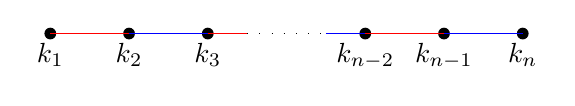
\begin{tikzpicture}
            \draw (0,0) node[circle, fill, inner sep=1.5pt]{};
            \draw (1,0) node[circle, fill, inner sep=1.5pt]{};
            \draw (2,0) node[circle, fill, inner sep=1.5pt]{};
            \draw (4,0) node[circle, fill, inner sep=1.5pt]{};
            \draw (5,0) node[circle, fill, inner sep=1.5pt]{};
            \draw (6,0) node[circle, fill, inner sep=1.5pt]{};
            \draw (0,0) node[below] {$k_1$};
            \draw (1,0) node[below] {$k_2$};
            \draw (2,0) node[below] {$k_3$};
            \draw (4,0) node[below] {$k_{n-2}$};
            \draw (5,0) node[below] {$k_{n-1}$};
            \draw (6,0) node[below] {$k_n$};
            \draw [red] (0,0)--(1,0);
            \draw [blue] (1,0)--(2,0);
            \draw [red] (2,0) --(2.5,0);
            \draw [loosely dotted] (2.5,0)--(3.5,0);
            \draw [blue] (3.5,0) --(4,0);
            \draw [red] (4,0)--(5,0);
            \draw [blue] (5,0)--(6,0);
        \end{tikzpicture}
        \caption{交错路径}
        \label{fig:cross-path}
    \end{figure}
    考虑作为端点的节点 $k_1$, 对于任意满足 $m\neq k_1,a_2=m^2+mk_1+k_1^2$ 的 $m$, 因为 $m\in \Gamma_{a_2}$, 所以 $m\notin \Gamma_{a_1}$. 由 $u(t_1+t,x_1-a_1t)=u(t_2+t,x_2-a_2t)=0$ 及定理 \ref{thm-3-3-1} 知 $c_m=0, d_{2,k_1}=0$. 而 $d_{2,k_1}$ 是所有满足 $m^2+mk_1+k_1^2=a_2$ 的数 $c_m e^{i(m^3t_2+mx_2)}$ 的和, 且其中 $m\neq k_1$ 的每一项都为零, 所以 $c_{k_1}=0$. 考虑节点 $k_2$, 以及任意满足 $m\neq k_1,a_1=m^2+mk_1+k_1^2$ 的 $m$. 已知 $m=k_1$ 的情形下 $c_{k_1}=0$, 此时便可将其视作只有蓝色线的端点, 再由同 $k_1$ 一样的论证可得 $c_{k_2}=0$. 依次进行下去, 可得路径上的节点的值全为 $0$.
    \item [(ii)] 仅存在长度等于 $3$ 的闭路径, 由引理 \ref{lma-3-3-2} 知必构成同色三角形. 不妨假设图 $G(a_1,a_2)$ 本身连通. 
    
    我们对图的节点个数 $n$ 进行归纳. 当 $n=3$ 时, $G(a_1,a_2)$ 是一个同色三角形, 不妨设颜色为红色, 则对该三角形的任意一个节点 $k$, 由 $u(t_1+t,x_1-a_1t)=u(t_2+t,x_2-a_2t)=0$ 及定理 \ref{thm-3-3-1} 可知满足 $m\neq k, a_2=m^2+mk+k^2$ 的 $m$ 满足 $c_m=0$, 再由 $d_{2,k}=\sum\limits_{a_2=m^2+mk+k^2,m\in\Z}c_m e^{i(m^3t_2+mx_2)}$ 可推出 $c_k=0$.
    当 $n=4$ 时, 必然是一个同色三角形与一个节点 $l$ 相连, 由于 $l$ 仅有一条边, 所以 $c_l=0$, 则可以将该图视作只有同色三角形的情形. 假设节点数为 $n-2,n-1$ 时, 可推出所有节点的值为 $0$, 现在我们考虑节点个数为 $n$ 的情形. 若存在一个端点, 即一个节点且只有一条边与其相连, 同样地则可以将其去掉, 则图可以视为节点个数 $n-1$ 的情形, 再利用归纳假设即可. 若不存在端点, 则必然存在同色三角形仅与一条边相连 (否则会出现长度大于 $3$ 的简单闭路径), 如图  \ref{no-end-points} 所示.
    \begin{figure}[htbp]
        \centering
        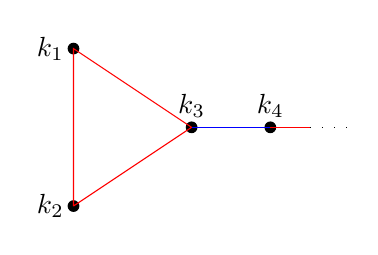
\begin{tikzpicture}
            \draw (-0.5,1) node[circle, fill, inner sep=1.5pt]{};
            \draw (-0.5,1) node[left] {$k_1$};
            \draw (-0.5,-1) node[circle, fill, inner sep=1.5pt]{};
            \draw (-0.5,-1) node[left] {$k_2$};
            \draw (1,0) node[circle, fill, inner sep=1.5pt]{};
            \draw (1,0) node[above] {$k_3$}; 
            \draw (2,0) node[circle, fill, inner sep=1.5pt]{};
            \draw (2,0) node [above] {$k_4$};
            \draw[red] (-0.5,-1)--(-0.5,1)--(1,0)--(-0.5,-1);
            \draw [blue] (1,0)--(2,0);
            \draw [red] (2,0) -- (2.5,0);
            \draw [loosely dotted] (2.5,0)--(3,0);
        \end{tikzpicture}
        \caption{不存在端点的情形}
        \label{no-end-points}
    \end{figure}
    由 $k_1$ 没有蓝色边可知, 对于任意满足 $m\neq k_1,a_2=m^2+mk_1+k_1^2$ 的 $m$, 由 $u(t_1+t,x_1-a_1t)=u(t_2+t,x_2-a_2t)=0$ 及定理 \ref{thm-3-3-1} 知 $c_m=0,d_{2,k_1}=0$. 再由 $d_{2,k_1}=\sum\limits_{a_2=m^2+mk_1+k_1^2,m\in\Z} c_me^{i(m^3t_2+mx_2)}$ 可推出 $c_{k_1}=0$. 同理可推出 $k_2=0$. 此时可将 $k_1,k_2$ 从图中去除, 则变成了节点个数为 $n-2$ 的图, 再利用归纳假设即可.   
\end{enumerate}

(2) $\Rightarrow$ (3). 考虑证明其逆否命题. 若存在长度大于 $3$ 的简单闭路径, 则其必为双色. 若不然, 则由引理 \ref{lma-3-3-2} 可知存在四个节点 $k_i,i=1,2,3,4$ 两两之间由相同颜色相连, 不妨设为红色, 则 $k_i^3-a_1 k_i=k_j^3-a_1k_j,\forall i,j$, 但这是不可能的. 再由引理 \ref{lma-3-3-3} 知存在简单交错闭路径, 设该交错闭路径为 $O(k_1,k_2,\cdots,k_{2n}), k_i\neq k_j, \forall i\neq j$. 不失一般性设 $k_1$ 与 $k_2$ 间的边为红色. 不妨令 $(t_0,x_0)=(t_1,x_1)=(t_2,x_2)$, 若不然, 则设 $(t_0,x_0)$ 为 $x=x_1-a_1(t-t_1)$ 与 $x=x_2-a_2(t-t_2)$ 的交点. 令 
\begin{equation*}
    u_0(x)=\sum_{j=1}^{2n}(-1)^je^{-i(k_j^3t_0+k_jx_0)}e^{ik_jx}.
\end{equation*}
则
\begin{equation*}
    u(t,x)=\sum_{j=1}^{2n}(-1)^j e^{-i(k_j^3t_0+k_jx_0)}e^{ik_j^3 t}e^{ik_jx} 
\end{equation*}
将 $(t,x)$ 由 $(t_0+t,x_0-a_1t)$ 代替可得对任意的 $t\in \R$ 有
\begin{align*}
    u(t_0+t,x_0-a_1t)&=\sum_{j=1}^{2n}(-1)^j e^{-i(k_j^3t_0+k_jx_0)}e^{ik_j^3 (t_0+t)}e^{ik_j(x_0-a_1t)} \\
    &=\sum_{j=1}^{2n}(-1)^j e^{i(k_j^3-a_1)t}\\
    &=\left(-e^{i(k_1^3-a_1 k_1)t)}+e^{i(k_2^3-a_2k_2)t)}\right)+\cdots\\
    &+\left(-e^{i(k_{2n-1}^3-a_1k_{2n-1})t)}+e^{i(k_{2n}^3-a_2k_{2n})t)}\right)\\
    &=0.
\end{align*}
上式最后一步用到了路径颜色的交错性.
同理对任意的 $t\in \R$, 有 
\begin{equation*}
    u(t_0+t,x_0-a_2t)=0.
\end{equation*}
然而 $\sum_{k\in \Z} |c_k|^2=2n$, 所以由解函数在两条线段上为零不可推出 $u_0=0$.

由 (1) $\Rightarrow$ (2) 显然, 所以最后只需要证明 (2) $\Rightarrow$ (1) 即可. 实际上, 这等价于证明
\begin{equation*}
    \sum_{k\in \Z} |c_k|^2\lesssim \sum_{k\notin \Pi_{a_1}\cap \Pi_{a_2}}|c_k|^2+\sum_{k\in \Pi_{a_1}\cap \Pi_{a_2}} |d_{1,k}|^2+|d_{2,k}|^2.
\end{equation*}
上式可化简为
\begin{equation}\label{final}
    \sum_{k\in \Pi_{a_1}\cap \Pi_{a_2}}|c_k|^2\lesssim \sum_{k\in \Pi_{a_1}\cap \Pi_{a_2}} |d_{1,k}|^2+|d_{2,k}|^2.
\end{equation}
我们使用反证法, 假设存在序列 $c_k^{(i)},i=1,2,\cdots,$ 使得当 $i\to \infty$ 时有
\begin{equation*}
    \frac{\sum_{k\in \Pi_{a_1}\cap \Pi_{a_2}} |d^{(i)}_{1,k}|^2+|d^{(i)}_{2,k}|^2}{ \sum_{k\in \Pi_{a_1}\cap \Pi_{a_2}}|c^{(i)}_k|^2}\longrightarrow 0.
\end{equation*}
由式 \ref{final} 的其次性, 可不失一般性, 设 $\sum_{k\in \Pi_{a_1}\cap \Pi_{a_2}}|c_k^{(i)}|^2=1, i=1,2,\cdots$. 由 $\Pi_{a_1}\cap \Pi_{a_2}$ 中元素只有有限个可知当 $i\to \infty$ 时 $d^{(i)}_{1,k}\to 0, d^{(i)}_{2,k}\to 0,\forall k\in \Pi_{a_1}\cap \Pi_{a_2}$. 设极限分别为 $c^{(0)}_k, d^{(0)}_{1,k}=d^{(0)}_{2,k}=0, \forall k\in \Pi_{a_1}\cap \Pi_{a_2}$, 且 
\begin{equation}\label{final-1}
    \sum_{k\in \Pi_{a_1}\cap \Pi_{a_2}}|c_k^{(0)}|^2=1.
\end{equation}
令 $u_0=\sum_{k\in \Pi_{a_1}\cap \Pi_{a_2}}c^{(0)}_k e^{ikx}$, 
从而由式 \eqref{final}可得 $c_k=0,\forall k\in \Pi_{a_1}\cap \Pi_{a_2}$, 这与式 \eqref{final-1} 相矛盾. 所以不等式 \eqref{obs-two-points} 成立.
\end{proof}
上面的定理是用边二染色图来刻画出能观测性, 由该定理可知, 给定任意两个不同速率的移动观测点, 能够建立相应能观测不等式当且仅当其在两条线段轨迹上有唯一延拓性. 另一方面, 为了验证其可观测性, 可通过作图 $G(a_1,a_2)$ 并尝试找到其长度大于 3 的简单闭回路. 

实际操作中, 定理 \ref{abstract-thm} 的刻画比较复杂, 接下来我们给出两个相对具体的判定方法. 第一个是利用 $a_1,a_2$ 的素因式分解, 第二个是利用函数 $y=x^3-ax$ 的增减性. 这两种方法在判别两个移动观测点的可观测性时更加简单.

\begin{theorem}\label{thm-use-prime}
给定任意的 $T>0$, 考虑方程 \eqref{kdv-r} 的解. 设 $a_1,a_2$ 为两个不同的正整数, $(t_1,x_1),(t_2,x_2)\in \R\times \T$. 若存在素数 $p\equiv 2\pmod{3}$ 使得 $\mathrm{deg}_p(a_1)\neq \mathrm{deg}_p(a_2)$, 则由
\begin{equation*}
    u(t_1+t,x_1-a_1t)=u(t_2+t,x_2-a_2t)=0,\quad \forall t\in (0,T)
\end{equation*}
可推出 $u$ 是平凡解, 即 $u_0=0$, 并且在该情形下存在不等式 \eqref{obs-two-points}.
\end{theorem}
\begin{proof}
不妨令 $\mathrm{deg}_p(a_1)>\mathrm{deg}_p(a_2),a_1,a_2\in \Gamma$, 由推论 \ref{crc-3-2-2} 可设 $\mathrm{deg}_p(a_1)=2e,e\in\N_{+}$, 则 $p^{2e}|a_1$. 令 $a_1=k^2+km+m^2,k\neq m$, 则 $a_1=(k-m\omega)(k-m\overline{\omega})$, 因为 $p\equiv 2\pmod{3}$, 由定理 \ref{thm-eisenstein} 知 $p$ 为 Eisenstein 素数, 则由唯一分解性质可得 $p^e | k-m\omega,p^e|k-m\overline{\omega}$, 进而有 $p^e|k, p^e|m$. 设 $k\in \Pi_{a_2}$, 则存在 $l\neq k$ 使得 $a_2=k^2+kl+l^2$ 成立. 由 $p^{2e}\nmid a_2$ 可得 $p^e\nmid k-l\omega,p^e\nmid k-l\overline{\omega}$, 再由 $p^e|k$ 可得 $p^e\nmid l$, 所以 $l\notin \Gamma_{a_1}$. 所以连接点 $k\in \Gamma_{a_1}$ 的边只能是红色边, 即 $k$ 是个孤立点, 孤立线段或孤立的红色三角形的一部分. 既然红色边都以这种形式存在, 则蓝色边也只会以孤立点, 孤立线段或孤立蓝色三角形的形式存在. 再由定理 \ref{abstract-thm} 的 (3) 可得结论. 
\end{proof}

\begin{theorem}\label{a24a1}
给定任意的 $T>0$, 考虑方程 \eqref{kdv-r} 的解. 设 $a_1,a_2$ 为两个不同的正整数, 且满足 $a_2>4a_1>0$, $(t_1,x_1), (t_2,x_2)\in \R\times \T$. 则由 
  \begin{equation*}
        u(t_1+t,x_1-a_1t)=u(t_2+t,x_2-a_2t)=0,\quad \forall t\in (0,T)
  \end{equation*}
可推出$u$ 是平凡解, 即 $u_0=0$, 并且在该情形下存在不等式 \eqref{obs-two-points}.
    \end{theorem}
    \begin{proof}
假设 $k\in  \Pi_{a_1}$. 此时只需要考虑 $k\in \left[0, 2\left(\frac{a_1}{3}\right)^{1 /2}\right]$ 的情形, 如图 \ref{fig6} 所示.
          \begin{figure}[htbp]
        \centering
         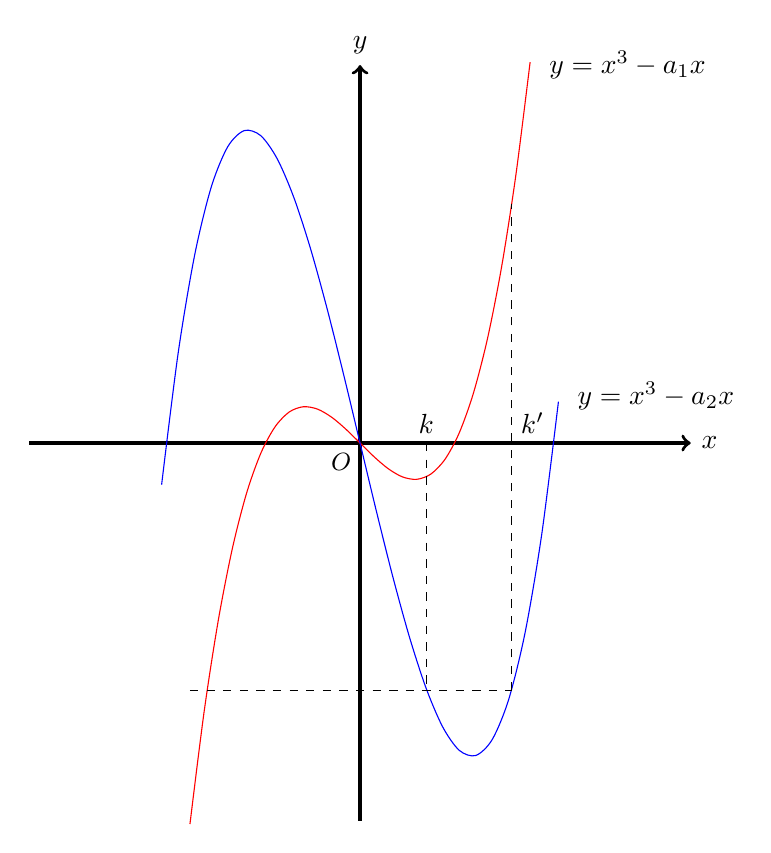
\begin{tikzpicture}[scale=1.2]
           % axes 
           \draw[very thick,->] (-3.5,0) -- (3.5,0) node[right] {$x$};
           \draw[very thick,->] (0,-4) -- (0,4) node[above] {$y$};
           \draw (-0.2,-0.01) node[below] {\small $O$};
           % functions
         \draw[red] plot[domain=-1.8:1.8, smooth] (\x, \x*\x*\x-1*\x);
         \draw[blue] plot[domain=-2.1:2.1, smooth] (\x, \x*\x*\x-4.2*\x);
         \draw[dashed] (0.7,0) node[above] {$k$} -- (0.7,-2.62);
         \draw[dashed] (-1.8,-2.62) -- (1.6,-2.62);
         \draw[dashed] (1.6,-2.62) -- (1.6,2.53);
         \draw (1.6,0) node[above right] {$k'$};
         \draw (1.9,4) node[right] {$y=x^3-a_1x$};
         \draw (2.2,0.5) node[right] {$y=x^3-a_2x$};
        \end{tikzpicture}
        \caption{函数$y=x^3-a_1x$ 和 $y=x^3-a_2 x$ 的图像.}
        \label{fig6}
    \end{figure}
     若 $k\in \Pi_{a_2} $, 则必然存在另一个不同的 $k'$ 使得 $k^3-a_2k={k'}^3-a_2k'$, 但是由函数图像可知 $|k'|\ge\left(\frac{a_2}{3}\right)^{1 /2}>2\left(\frac{a_2}{3}\right)^{1 /2}$, 所以 $k'\notin \Pi_{a_1}$. 由定义式
     \begin{equation*}
         d_{2,k}=\sum\limits_{\substack{k'\neq k\in \Z,\\ k^2+mk+m^2=a_2}} c_{k'}e^{i(k'^3t_2+k'x_0)}+c_k e^{i(k^3t_2+kt_2)}
     \end{equation*}
     以及条件 $u(t_1+t,x_1-a_1t)=u(t_2+t,x_2-a_2t)=0,\forall t\in (0,T)$ 可得 $$\sum\limits_{\substack{k'\neq k\in \Z,\\ k^2+mk+m^2=a_2}} c_{k'}e^{i(k'^3t_2+k'x_0)}=0$$ 以及 $d_{2,k}=0$, 进而 $c_k=0$. 所以 $u_0=0$. 再由定理 \ref{abstract-thm} 可知不等式 \eqref{obs-two-points} 成立.
      \end{proof}
\iffalse      
\begin{theorem}
给定任意的 $T>0$ , 考虑方程 \eqref{kdv-r} 的解. 设 $n\ge 3$ 个不同的实数 $a_1<a_2<\cdots <a_n$, $(t_i,x_i)\in \R\times \T, i=1,2,\cdots,n$. 则由
\begin{equation*}
    u(t_1+t,x_1-a_1t)=u(t_2+t,x_2-a_2t)=\cdots=u(t_n+t,x_n-a_nt)=0,\quad \forall t\in (0,T)
\end{equation*}
可推出 $u$ 是平凡解, 即 $u_0=0$, 并且在该情形下不等式 
\begin{equation}
    \sum_{k\in\Z}|c_k|^2\lesssim \int_{0}^T\sum_{i=1}^n|u(t_i+t,x_i-a_i t)|\d t
\end{equation}
成立.
\end{theorem}
\begin{proof}
不妨令 $a_i\in \Gamma, a_i>0, \forall i=1,2,\cdots,n$. 若 $a_n>4a_1$, 则可由定理 \ref{a24a1} 直接推出结论. 

设 $a_n\le 4a_1$, 则由定理 \ref{thm-use-prime} 可知对任意的素数 $p\equiv 2\pmod{3}$, $\mathrm{deg}_p(a_i)=\mathrm{deg}_p(a_j),\forall i\neq j$. 所以不妨令所有的 $a_i$ 都不存在模 $3$ 余 $2$ 的素因子. 
\end{proof}

\fi

   

